\chapter{دورات حياة النباتات اليابسة وتكاثرها}\label{ch:b2:plant-life-cycles}

الوسادة الخضراء من \omterm{def:b2:plant-life-cycles:moss}{الطحلب} على جدار نبات واحد؛ أما السوق البنية
الناهضة منها في الربيع، وعلى كل منها محفظة أبواغ، فنبات آخر --- فرد
مختلف، بضعفي عدد الصبغيات، ينمو من الأول ويعيش عليه. وسعفة \omterm{def:b2:plant-life-cycles:fern}{سرخس}
تحمل أبواغًا على وجهها السفلي، لكن الأبواغ لا تنمو سراخس: بل تنمو
حرشفة خضراء قلبية الشكل عرضها بضعة مليمترات، وفيها تُصنع النطاف
والبويضات، ومن تلك الحرشفة ينبثق \omterm{def:b2:plant-life-cycles:fern}{سرخس} جديد. وكل نبات يابس يناوب على
هذا النحو بين جسمين، أحدهما \omterm{def:b2:meiosis-heredity:meiosis}{فردي الصيغة} والآخر ثنائيها. يتتبع هذا
الفصل التناوب من الطحالب إلى البذرة، ويبين كيف حررت سلسلة من
التغيرات فيه --- انكماش الجسم \omterm{def:b2:meiosis-heredity:meiosis}{الفردي الصيغة}، وابتكار حبوب \omterm{def:b2:plant-life-cycles:heterospory}{اللقاح}،
وإحاطة \omterm{def:b2:plant-life-cycles:heterospory}{البييضة}، والبذرة --- التكاثرَ من الماء، ومكّنت النباتات من
تغطية القارات.

\section{ثلاثة أنماط من دورة الحياة}

\begin{definition}[فردي الصيغة، ثنائي الصيغة، فردي--ثنائي الصيغة]\label{def:b2:plant-life-cycles:cycles}
\index{دورة حياة}\index{تناوب الأجيال}\index{طور مشيجي}\index{طور بوغي}
كل دورة حياة جنسية تحوي \emph{إلقاحًا} واحدًا يضاعف عدد الصبغيات،
و\emph{تقسمًا منصّفًا} واحدًا ينصّفه؛ وتختلف الدورات فيما يقع بينهما.
ففي الدورة \emph{فردية الصيغة} تكون اللاقحة الخلية الثنائية الصيغة
الوحيدة وتخضع \omterm{def:b2:meiosis-heredity:meiosis}{للتقسم المنصّف} حالًا؛ فالكائن \omterm{def:b2:meiosis-heredity:meiosis}{فردي الصيغة} وأعراسه
تُصنع بالتقسم الخيطي (\emph{Chlamydomonas}، وكثير من الطحالب
والفطريات). وفي الدورة \emph{ثنائية الصيغة} يصنع \omterm{def:b2:meiosis-heredity:meiosis}{التقسم المنصّف}
الأعراس مباشرة، فتكون الأعراس الخلايا الفردية الصيغة الوحيدة، ويكون
الكائن \omterm{def:b2:meiosis-heredity:meiosis}{ثنائي الصيغة} (الحيوانات، \omterm{def:b2:plant-life-cycles:moss}{والطحلب} البني \emph{Fucus}). وفي
الدورة \emph{الفردية--الثنائية الصيغة} يصنع \omterm{def:b2:meiosis-heredity:meiosis}{التقسم المنصّف}
\emph{أبواغًا} تنمو بالتقسم الخيطي إلى كائن \omterm{def:b2:meiosis-heredity:meiosis}{فردي الصيغة} هو
\emph{الطور المشيجي}، يصنع الأعراس بالتقسم الخيطي؛ وتنمو اللاقحة
بالتقسم الخيطي إلى كائن \omterm{def:b2:meiosis-heredity:meiosis}{ثنائي الصيغة} هو \emph{الطور البوغي}، يصنع
الأبواغ \omterm{def:b2:meiosis-heredity:meiosis}{بالتقسم المنصّف}. فيتناوب جسمان عديدا الخلايا --- وهو
\emph{تناوب الأجيال} --- وهذه دورة كل نبات يابس وكثير من الطحالب.
\end{definition}

\begin{omfigure}
\begin{tikzpicture}[every node/.style={font=\scriptsize}, >=stealth]
  \foreach \dx/\title/\hap/\dip in {0/{فردية الصيغة (\emph{Chlamydomonas})}/{كائن فردي الصيغة ($n$)}/{لاقحة ($2n$)}, 5.2/{ثنائية الصيغة (الحيوانات)}/{أعراس ($n$)}/{كائن ثنائي الصيغة ($2n$)}, 10.4/{فردية--ثنائية الصيغة (النباتات)}/{طور مشيجي ($n$)}/{طور بوغي ($2n$)}} {
    \begin{scope}[xshift=\dx cm]
      \node[anchor=south, font=\scriptsize\bfseries] at (2,2.5) {\title};
      \draw[thick, omDef, ->] (0.6,0.4) arc (200:340:1.5 and 1.0);
      \draw[thick, omThm, ->] (3.4,1.4) arc (20:160:1.5 and 1.0);
      \node[omDef, anchor=north] at (2,-0.3) {\hap};
      \node[omThm, anchor=south] at (2,2.05) {\dip};
      \node[anchor=south west] at (3.4,1.05) {إلقاح};
      \node[anchor=north east] at (0.55,0.75) {تقسم منصّف};
    \end{scope}
  }
  % emphasise the dominant phase by thickness of the arcs: draw thicker arcs
  \draw[line width=2.4pt, omDef, ->] (0.6,0.4) arc (200:340:1.5 and 1.0);
  \draw[line width=2.4pt, omThm, ->] (5.2+3.4,1.4) arc (20:160:1.5 and 1.0);
  \draw[line width=2.4pt, omDef, ->] (10.4+0.6,0.4) arc (200:340:1.5 and 1.0);
  \draw[line width=2.4pt, omThm, ->] (10.4+3.4,1.4) arc (20:160:1.5 and 1.0);
\end{tikzpicture}

{\small ثلاث دورات حياة. بالأزرق: الطور \omterm{def:b2:meiosis-heredity:meiosis}{الفردي الصيغة}؛ وبالأحمر:
الطور \omterm{def:b2:meiosis-heredity:meiosis}{الثنائي الصيغة}؛ والأقواس السميكة هي الأجسام العديدة الخلايا.
وكل دورة تمر مرة \omterm{def:b2:meiosis-heredity:meiosis}{بالتقسم المنصّف} ومرة بالإلقاح؛ وإنما تختلف في أي
طور --- أو كليهما --- ينمو كائنًا.}
\end{omfigure}

\begin{proposition}[ما يعنيه تناوب الأجيال]\label{prop:b2:plant-life-cycles:alternation}
في النبات اليابس يكون الجيلان كائنين اثنين لا مرحلتين من كائن واحد:
فللطور المشيجي \omterm{def:b2:plant-life-cycles:cycles}{والطور البوغي} مورثومان مختلفان (\omterm{def:b2:meiosis-heredity:meiosis}{فردي الصيغة} وثنائيها)،
وجسمان مختلفان، وقياسان يختلفان غالبًا برتب من القدر، وينمو كل
منهما بالتقسم الخيطي من خلية واحدة --- بوغ أو لاقحة. ويصنع \omterm{def:b2:plant-life-cycles:cycles}{الطور
المشيجي} الأعراس في أعضاء عديدة الخلايا هي \emph{المذاري} (النطاف)
و\emph{الأرحام} (بويضة واحدة في كل منها، في قارورة تسبح النطفة في
عنقها نزولًا)؛ ويصنع \omterm{def:b2:plant-life-cycles:cycles}{الطور البوغي} الأبواغ في \emph{حوافظ بوغية}.
ويتحول الميزان عبر النباتات اليابسة: ففي الطحالب يكون \omterm{def:b2:plant-life-cycles:cycles}{الطور المشيجي}
هو النبات \omterm{def:b2:plant-life-cycles:cycles}{والطور البوغي} ساقًا تابعة؛ وفي السراخس يكون \omterm{def:b2:plant-life-cycles:cycles}{الطور البوغي}
هو النبات \omterm{def:b2:plant-life-cycles:cycles}{والطور المشيجي} حرشفة حرة؛ وفي النباتات البذرية ينكمش \omterm{def:b2:plant-life-cycles:cycles}{الطور
المشيجي} إلى بضع خلايا مختبئة داخل أنسجة \omterm{def:b2:plant-life-cycles:cycles}{الطور البوغي} --- أي حبة
\omterm{def:b2:plant-life-cycles:heterospory}{اللقاح} ومحتويات \omterm{def:b2:plant-life-cycles:heterospory}{البييضة}.
\end{proposition}
\begin{proof}[شواهد]
أنبت هوفمايستر (1851) أبواغ الطحالب والسراخس وذنب الخيل وشوكران
الأرض، وتتبع نمو الأجسام الخضراء الصغيرة التي أنتجتها، فوجد عليها
المذاري والأرحام، وراقب الجنين ينمو من البويضة الملقحة داخل الرحم
إلى النبات الحامل للأبواغ. ثم بيّن أن \omterm{def:b2:plant-life-cycles:heterospory}{بييضة} صنوبر تحوي البنى نفسها
مختزلة --- أرحامًا داخل نسيج هو \omterm{def:b2:plant-life-cycles:cycles}{طور مشيجي} مستبقى --- وأن الطحالب
والسراخس والنباتات البذرية سلسلة واحدة بدورة واحدة. أما عدّ
الصبغيات الذي فسّر الجيلين (شتراسبورغر، 1894) فجاء بعد أربعين سنة.
\end{proof}

\section{الطحالب: الطور المشيجي هو النبات}

\begin{definition}[دورة حياة الطحلب]\label{def:b2:plant-life-cycles:moss}
\index{طحلب}\index{خيط أولي}\index{رحم}\index{مذراة}
ينبت \emph{بوغ} الطحلب خيطًا أخضر متفرعًا هو \emph{الخيط الأولي}،
تنمو منه براعم إلى سوق مورقة --- وهي \emph{\omterm{def:b2:plant-life-cycles:cycles}{الطور المشيجي}}، بطول بضعة
سنتيمترات، بلا جذور حقيقية ولا خشب ولا لحاء، تثبته أشباه جذور
ويمتص الماء بسطحه كله. ويحمل عند أطراف السوق \emph{مذاري} تطلق
نطافًا ثنائية السوط في غشاء من مطر أو ندى، و\emph{أرحامًا} في كل
منها بويضة واحدة عند قاعدة عنق؛ وتسبح النطاف بضعة سنتيمترات على
الأكثر، تهديها جاذبات كيميائية، فتلقّح البويضة في مكانها. وتنمو
اللاقحة إلى \emph{\omterm{def:b2:plant-life-cycles:cycles}{الطور البوغي}}: قدم مغروسة في \omterm{def:b2:plant-life-cycles:cycles}{الطور المشيجي}، وساق
(\emph{سويقة})، و\emph{محفظة} يصنع فيها \omterm{def:b2:meiosis-heredity:meiosis}{التقسم المنصّف} عشرات آلاف
الأبواغ، تُطلق عبر حلقة من أسنان تتحسس الرطوبة وتنفتح في الهواء
الجاف. \omterm{def:b2:plant-life-cycles:cycles}{والطور البوغي} يركّب ضوئيًا قليلًا لكن \omterm{def:b2:plant-life-cycles:cycles}{الطور المشيجي} يغذيه
عبر قدمه، وهو لا يعيش وحده أبدًا.
\end{definition}

\begin{omfigure}
\begin{tikzpicture}[every node/.style={font=\scriptsize}, >=stealth]
  \node[draw, rounded corners, fill=omDef!12, align=center] (spore) at (0,3) {بوغ ($n$)};
  \node[draw, rounded corners, fill=omDef!12, align=center] (proto) at (3.2,3) {خيط أولي};
  \node[draw, rounded corners, fill=omDef!12, align=center] (gam) at (6.6,3) {طور مشيجي مورق ($n$)\\مذارٍ وأرحام};
  \node[draw, rounded corners, fill=omDef!12, align=center] (gametes) at (11.2,3) {نطفة وبويضة ($n$)};
  \node[draw, rounded corners, fill=omThm!12, align=center] (zyg) at (11.2,0.8) {لاقحة ($2n$)};
  \node[draw, rounded corners, fill=omThm!12, align=center] (sporo) at (6.6,0.8) {طور بوغي ($2n$)\\قدم وسويقة ومحفظة};
  \node[draw, rounded corners, fill=omThm!12, align=center] (cap) at (2.4,0.8) {تقسم منصّف في المحفظة};
  \draw[->, thick] (spore) -- (proto) node[midway, above] {تقسم خيطي};
  \draw[->, thick] (proto) -- (gam);
  \draw[->, thick] (gam) -- (gametes) node[midway, above] {تقسم خيطي};
  \draw[->, thick] (gametes) -- (zyg) node[pos=0.3, right, align=left] {إلقاح\\في غشاء ماء};
  \draw[->, thick] (zyg) -- (sporo) node[midway, above] {تقسم خيطي};
  \draw[->, thick] (sporo) -- (cap);
  \draw[->, thick] (cap) -| (spore) ;
  \node[omDef, anchor=west] at (-1.9,3.9) {فردي الصيغة};
  \node[omThm, anchor=west] at (-1.9,-0.1) {ثنائي الصيغة};
  \draw[gray, dashed] (-1.9,1.9) -- (13.2,1.9);
\end{tikzpicture}

{\small دورة \omterm{def:b2:plant-life-cycles:moss}{الطحلب}. النبات المورق هو \omterm{def:b2:plant-life-cycles:cycles}{الطور المشيجي} \omterm{def:b2:meiosis-heredity:meiosis}{الفردي الصيغة}؛
\omterm{def:b2:plant-life-cycles:cycles}{والطور البوغي} ساق ومحفظة تنمو عليه، يغذيها، وتصنع الأبواغ \omterm{def:b2:meiosis-heredity:meiosis}{بالتقسم
المنصّف}.}
\end{omfigure}

\begin{omfigure}
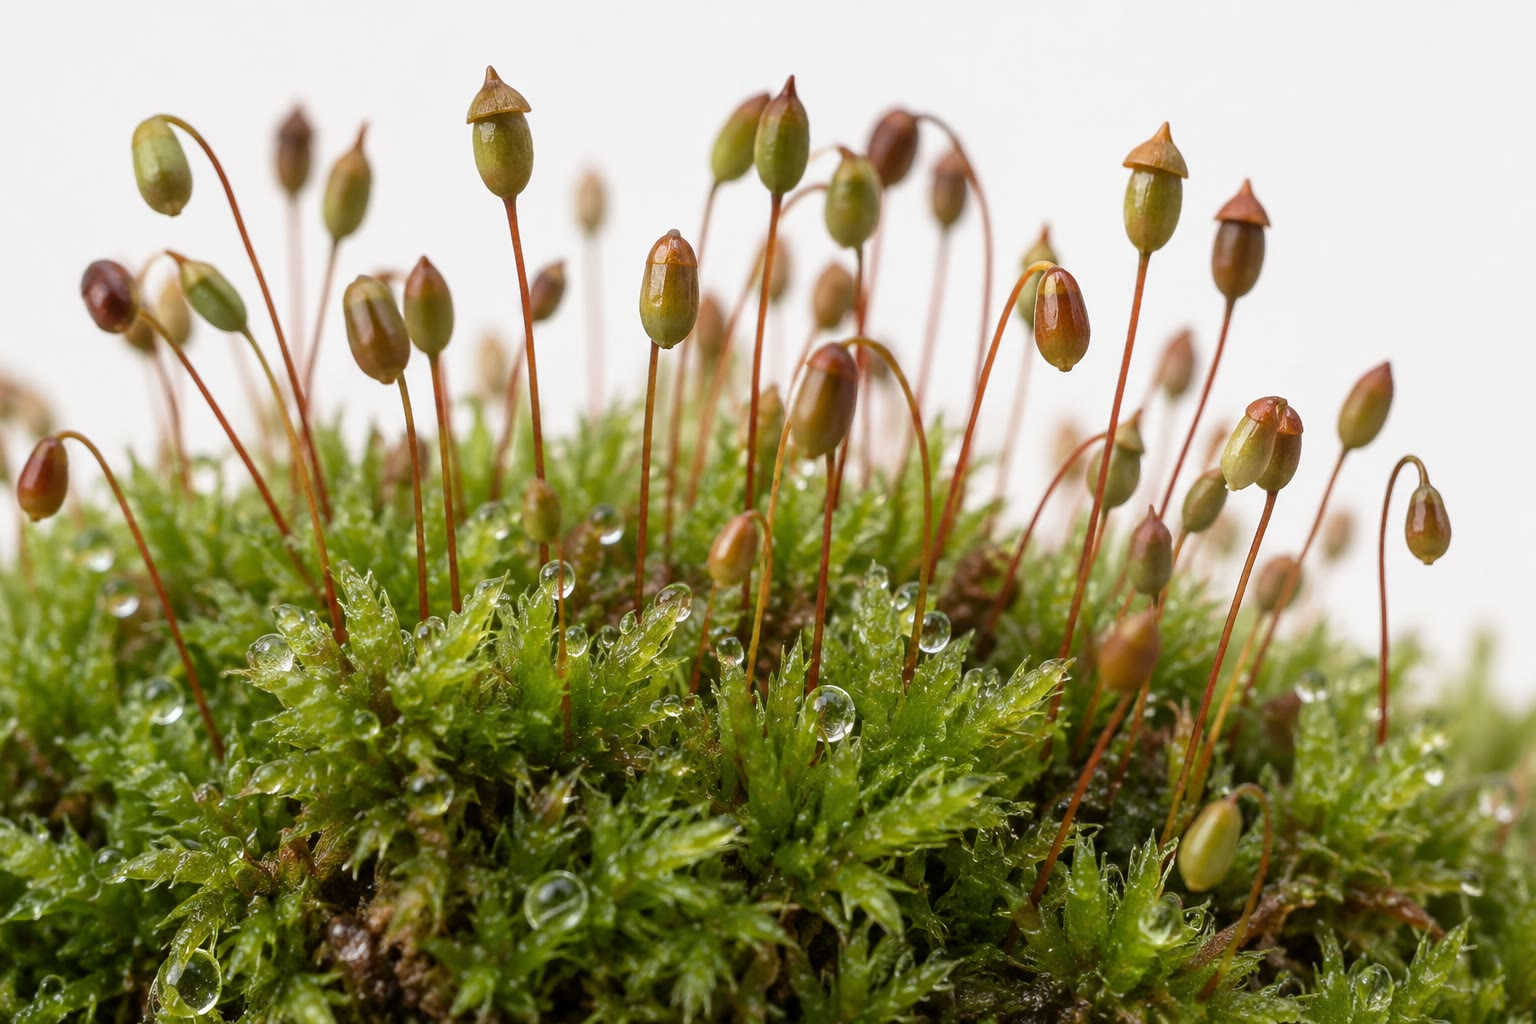
\includegraphics[width=0.6\linewidth]{images/book4/ai/b4-05-moss-sporophytes.jpg}

{\small وسادة \omterm{def:b2:plant-life-cycles:moss}{طحلب} في الربيع: السوق الخضراء هي الأطوار المشيجية،
وكل ساق محمرّة بمحفظتها \omterm{def:b2:plant-life-cycles:cycles}{طور بوغي} نما من بويضة ملقحة، ولا يزال
متصلًا بالساق التي صنعت البويضة.}
\end{omfigure}

\begin{example}[كلفة النطاف السابحة]\label{ex:b2:plant-life-cycles:sperm}
تسبح نطفة \omterm{def:b2:plant-life-cycles:moss}{الطحلب} بنحو \qty{100}{\micro m/s}؛ ولتبلغ رحمًا يبعد
\qty{2}{cm} تحتاج إلى \qty{200}{s} من غشاء ماء متصل --- رشة مطر، أو
ندى غزير. فالإلقاح إذن محصور في الطقس الرطب وفي المسافات القصيرة،
ومعظم الطحالب والسراخس وأقاربها تعيش في أماكن ندية أو تتكاثر في
الموسم الرطب؛ ومذاري بعض الطحالب تجلس في كأس رشّ يقذف شكله قطرات
المطر، والنطاف التي تحملها، نصف متر. وهذه هي التبعية التي أفلتت
منها النباتات البذرية.
\end{example}

\section{السراخس: الطور البوغي هو النبات}

\begin{definition}[دورة حياة السرخس]\label{def:b2:plant-life-cycles:fern}
\index{سرخس}\index{مشيجة}\index{بثرة}\index{حافظة بوغية}
السرخس هو \emph{\omterm{def:b2:plant-life-cycles:cycles}{الطور البوغي}}: جذمور بجذور وخشب ولحاء وسعف. وعلى
الوجه السفلي للسعف الخصبة، تصنع عناقيد من \emph{الحوافظ البوغية}
(\emph{بثرات}، تحت غطاء واقٍ غالبًا) 64 بوغًا \omterm{def:b2:meiosis-heredity:meiosis}{بالتقسم المنصّف} في كل
حافظة، وتقذفها بانفلات حلقة من الخلايا سميكة الجدر وهي تجف. والبوغ
الذي يحط على تربة ندية ينمو \emph{مشيجة}: طورًا مشيجيًا أخضر قلبي
الشكل عرضه بضعة مليمترات، بسمك خلية واحدة، بأشباه جذور، يعيش حرًا
بضعة أسابيع. ويحمل مذاري وأرحامًا على وجهه السفلي؛ وتسبح النطاف في
غشاء ماء التربة إلى البويضة؛ وتنمو اللاقحة طورًا بوغيًا فتيًا يأخذ
غذاءه الأول من المشيجة ثم يتجذر، فتموت المشيجة. والجيلان مستقلان
كلاهما، لكنهما غير متكافئين: \omterm{def:b2:plant-life-cycles:cycles}{فالطور البوغي} يعيش عقودًا وقد يبلغ
أمتارًا، \omterm{def:b2:plant-life-cycles:cycles}{والطور المشيجي} يعيش أسابيع ويبلغ مليمترات.
\end{definition}

\begin{omfigure}
\begin{tikzpicture}[every node/.style={font=\scriptsize}, >=stealth]
  \node[draw, rounded corners, fill=omThm!12, align=center] (fern) at (0,3) {نبات السرخس، الطور البوغي ($2n$)\\جذور وجذمور وسعف};
  \node[draw, rounded corners, fill=omThm!12, align=center] (sor) at (5.4,3) {حوافظ بوغية في بثرات\\(تحت السعف)};
  \node[draw, rounded corners, fill=omDef!12, align=center] (spore) at (10.4,3) {أبواغ ($n$)\\64 في الحافظة};
  \node[draw, rounded corners, fill=omDef!12, align=center] (pro) at (10.4,0.6) {مشيجة ($n$)\\حرة، بقياس المليمتر\\مذارٍ وأرحام};
  \node[draw, rounded corners, fill=omDef!12, align=center] (gam) at (5.4,0.6) {نطفة وبويضة ($n$)};
  \node[draw, rounded corners, fill=omThm!12, align=center] (zyg) at (0,0.6) {لاقحة ($2n$)، ثم\\طور بوغي فتي\\على المشيجة};
  \draw[->, thick] (fern) -- (sor);
  \draw[->, thick] (sor) -- (spore) node[midway, above] {تقسم منصّف};
  \draw[->, thick] (spore) -- (pro) node[midway, right] {تقسم خيطي};
  \draw[->, thick] (pro) -- (gam) node[midway, above] {تقسم خيطي};
  \draw[->, thick] (gam) -- (zyg) node[midway, above, align=center] {إلقاح\\(بنطاف سابحة)};
  \draw[->, thick] (zyg) -- (fern) node[midway, right] {تقسم خيطي};
  \draw[gray, dashed] (7.9,-0.5) -- (7.9,4.0);
  \node[omThm, anchor=south] at (2.7,3.9) {الجيل الثنائي الصيغة};
  \node[omDef, anchor=south] at (10.4,3.9) {الجيل الفردي الصيغة};
\end{tikzpicture}

{\small دورة \omterm{def:b2:plant-life-cycles:fern}{السرخس}. النبات الذي نسميه سرخسًا هو \omterm{def:b2:plant-life-cycles:cycles}{الطور البوغي}
\omterm{def:b2:meiosis-heredity:meiosis}{الثنائي الصيغة}؛ \omterm{def:b2:plant-life-cycles:cycles}{والطور المشيجي} \omterm{def:b2:meiosis-heredity:meiosis}{الفردي الصيغة} \omterm{def:b2:plant-life-cycles:fern}{مشيجة} قصيرة العمر تسبح
عليها النطاف إلى البويضات.}
\end{omfigure}

\begin{omfigure}
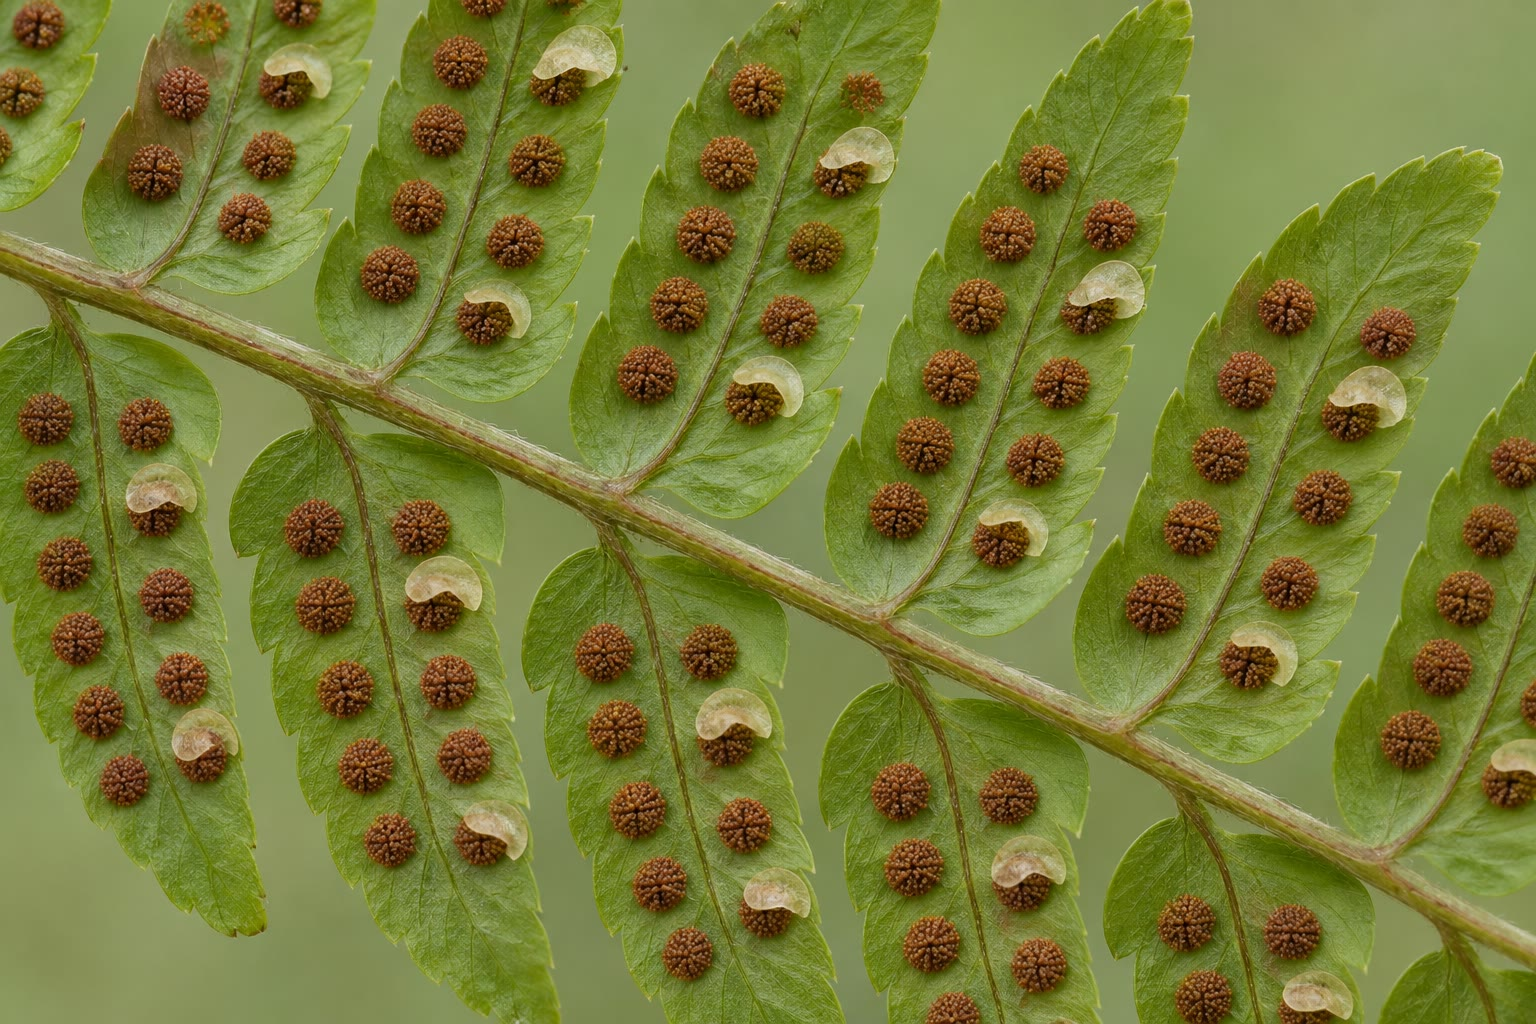
\includegraphics[width=0.6\linewidth]{images/book4/ai/b4-05-fern-sori.jpg}

{\small الوجه السفلي لسعفة \omterm{def:b2:plant-life-cycles:fern}{سرخس} خصبة: كل نقطة بنية \omterm{def:b2:plant-life-cycles:fern}{بثرة}، أي عنقود
من الحوافظ البوغية، وبعضها لا يزال مغطى بالغطاء الذي يحميها حتى
تنضج.}
\end{omfigure}

\begin{theorem}[انتشار البوغ]\label{thm:b2:plant-life-cycles:dispersal}
\index{انتشار الأبواغ}
بوغ نصف قطره $r$ وكثافته $\rho_s$ يُطلق من ارتفاع $h$
في رياح أفقية سرعتها $u$ يهبط بسرعة ستوكس الحدية
$v_s = 2r^2(\rho_s - \rho_{\text{الهواء}})g/9\eta_{\text{الهواء}}$
ويحط، في هواء مطبق ساكن، على مسافة
\[
x = \frac{u\,h}{v_s}
\]
من النبات. وبوغ \omterm{def:b2:plant-life-cycles:fern}{سرخس} نصف قطره \qty{15}{\micro m} وكثافته
\qty{1100}{kg/m^3} ($\eta_{\text{الهواء}} = \qty{1.8e-5}{Pa.s}$)
يهبط بسرعة \qty{3}{cm/s}؛ وينتقل من سعفة على \qty{0.5}{m} في رياح
سرعتها \qty{2}{m/s} نحو \qty{30}{m}، وفي هواء يوم عاصف المضطرب،
الذي يرفع كسرًا من الأبواغ إلى ما فوق ارتفاع الإطلاق بكثير، ينتقل
قليل منها مئات الكيلومترات --- ولهذا كانت فلورا السراخس في الجزر
المحيطية غنية وفلورا نباتاتها البذرية فقيرة.
\end{theorem}
\begin{proof}
زمن السقوط هو $h/v_s$ (إذ يبلغ البوغ سرعته الحدية في
ميكروثوانٍ)، وتحمله الرياح خلاله مسافة $u\,h/v_s$. أما السرعة
الحدية فتنجم عن موازنة جرّ ستوكس $6\pi\eta r
v_s$ بالوزن ناقص قوة الطفو $\tfrac43\pi r^3(\rho_s -
\rho_{\text{الهواء}})g$، كما في \cref{ch:b2:unicellular-diversity}.
\end{proof}

\section{النباتات البذرية: الطور المشيجي مختبئ}

\begin{definition}[تغاير الأبواغ، وحبة اللقاح، والبييضة]\label{def:b2:plant-life-cycles:heterospory}
\index{تغاير الأبواغ}\index{حبة لقاح}\index{بييضة}\index{بوغ صغير}\index{بوغ كبير}
الطحالب ومعظم السراخس \emph{متماثلة الأبواغ}: صنف واحد من الأبواغ،
وصنف واحد من الأطوار المشيجية يحمل الجنسين. أما النباتات البذرية
(وقليل من السراخس وشوكران الأرض) فهي \emph{متغايرة الأبواغ}: فالأبواغ
\emph{الصغيرة}، وهي صغيرة كثيرة، تنمو أطوارًا مشيجية ذكرية؛
والأبواغ \emph{الكبيرة}، وهي كبيرة قليلة، تنمو أطوارًا أنثوية. وفي
النباتات البذرية ينكمش الطوران إلى لا شيء تقريبًا ولا يغادر أي
منهما أنسجة \omterm{def:b2:plant-life-cycles:cycles}{الطور البوغي} وحده. \omterm{def:b2:plant-life-cycles:cycles}{والطور المشيجي} الذكري هو \emph{حبة
اللقاح}: بوغ صغير انقسم مرتين أو ثلاثًا داخل جداره، تحمله الرياح أو
الحيوانات إلى العضو الأنثوي، حيث ينمي \emph{أنبوب لقاح}
ويسلّم نطافه --- بلا حاجة إلى ماء. أما \omterm{def:b2:plant-life-cycles:cycles}{الطور المشيجي} الأنثوي فينمو
داخل \omterm{def:b2:plant-life-cycles:fern}{الحافظة البوغية} الكبيرة، وهي تبقى على الأم محاطة بغلاف
\emph{ركامي} واحد أو اثنين وفيهما ثقب هو \emph{النقير}: والبنية كلها
هي \emph{البييضة}. وبعد الإلقاح تصير البييضة \emph{بذرة}: جنين \omterm{def:b2:plant-life-cycles:cycles}{طور
بوغي}، ومخزون غذاء، وقشرة مصنوعة من الغلافين، ساكنة حتى تصير الظروف
مواتية.
\end{definition}

\begin{omfigure}
\begin{tikzpicture}[every node/.style={font=\scriptsize}]
  % ovule in section
  \draw[thick, fill=omExo!25] (0,0) ellipse (1.6 and 2.2);
  \draw[thick, fill=omExo!10] (0,0) ellipse (1.25 and 1.85);
  \draw[thick, fill=white] (0,-0.15) ellipse (0.8 and 1.3);
  \draw[thick, fill=omDef!25] (0,0.6) ellipse (0.45 and 0.55);
  \fill[omDef!80!black] (0,0.75) circle (0.12);
  % micropyle: gap at top
  \fill[white] (-0.35,1.7) rectangle (0.35,2.35);
  \draw[thick] (-0.35,1.7) -- (-0.35,2.2); \draw[thick] (0.35,1.7) -- (0.35,2.2);
  \draw[thick] (-0.35,2.2) arc (180:90:0.1) ; \draw[thick] (0.35,2.2) arc (0:90:0.1);
  % pollen grain and tube
  \draw[thick, fill=omProp!40] (0.9,3.0) circle (0.22);
  \draw[thick, omProp] (0.75,2.85) .. controls (0.2,2.6) and (0.05,2.0) .. (0.05,1.25);
  % stalk
  \draw[thick] (0,-2.2) -- (0,-2.8);
  % labels
  \draw (1.45,-0.9) -- (2.6,-0.9) node[right] {الغلاف (أو الغلافان)};
  \draw (1.0,-0.6) -- (2.6,-1.5) node[right] {حافظة بوغية كبيرة (نوسيلة)};
  \draw (0.55,-1.0) -- (2.6,-2.1) node[right, align=left] {طور مشيجي أنثوي\\(من بوغ كبير واحد)};
  \draw (0.35,0.45) -- (2.6,0.3) node[right] {رحم};
  \draw (0.1,0.78) -- (2.6,1.0) node[right] {بويضة};
  \draw (0.35,2.0) -- (2.6,2.0) node[right] {نقير};
  \draw (1.1,3.0) -- (2.6,3.0) node[right] {حبة لقاح وأنبوب لقاح};
  \node[right] at (0.1,-2.6) {حامل};
\end{tikzpicture}

{\small \omterm{def:b2:plant-life-cycles:heterospory}{بييضة} عاريات البذور في مقطع. \omterm{def:b2:plant-life-cycles:cycles}{الطور المشيجي} الأنثوي، النامي
من \omterm{def:b2:plant-life-cycles:heterospory}{بوغ كبير} واحد داخل \omterm{def:b2:plant-life-cycles:fern}{الحافظة البوغية} الكبيرة، ملفوف في غلاف ذي
ثقب؛ وحبة \omterm{def:b2:plant-life-cycles:heterospory}{اللقاح}، الملتقطة عند النقير، تنمي أنبوبًا إلى البويضة.
وبعد الإلقاح يصير الكل بذرة.}
\end{omfigure}

\begin{proposition}[دورة الصنوبريات]\label{prop:b2:plant-life-cycles:conifer}
\index{صنوبري}\index{مخروط}\index{بذرة}
يحمل الصنوبر صنفين من المخاريط. \emph{فالمخاريط الذكرية} الصغيرة،
في عناقيد في الربيع، تحوي حوافظ بوغية صغيرة يصنع فيها \omterm{def:b2:meiosis-heredity:meiosis}{التقسم المنصّف}
أبواغًا صغيرة؛ وينقسم كل منها إلى حبة \omterm{def:b2:plant-life-cycles:heterospory}{لقاح} رباعية الخلايا بمثانتي
هواء، وتُطلق بالملايين في الرياح. و\emph{المخاريط الأنثوية} تحمل
بييضتين على الوجه العلوي لكل حرشفة. \omterm{def:b2:plant-life-cycles:heterospory}{واللقاح} الذي تهبّ به الرياح بين
الحراشف تجذبه قطرة سائل إلى النقير؛ ثم ينمو \omterm{def:b2:plant-life-cycles:cycles}{الطور المشيجي} الأنثوي،
الذي لم يكن قد نما بعد، خلال السنة التالية من \omterm{def:b2:plant-life-cycles:heterospory}{البوغ الكبير} الوحيد
الباقي إلى نسيج من بضعة آلاف خلية فيه رحمان أو ثلاثة؛ وينمو أنبوب
\omterm{def:b2:plant-life-cycles:heterospory}{لقاح} ببطء عبر النوسيلة، ويسلّم، بعد خمسة عشر شهرًا من الإلقاح
اللقاحي، نطفة إلى بويضة. وينمو الجنين في \omterm{def:b2:plant-life-cycles:cycles}{الطور المشيجي} الذي يصير
مخزون غذاء البذرة؛ وتُطلق البذرة المجنحة في الخريف الثاني حين ينفتح
المخروط. فالبذور تستغرق سنوات وتكلف كثيرًا؛ وهي في المقابل تنتشر
جافة، وتنجو من الشتاء والجفاف، وتحمل غذاء البادرة لأسابيعها الأولى.
\end{proposition}

\begin{omfigure}
\begin{tikzpicture}[every node/.style={font=\scriptsize}, >=stealth]
  \draw[thick, ->] (0,0) -- (13.2,0);
  \foreach \x/\l in {0/{ربيع السنة 1}, 4.4/{ربيع السنة 2}, 8.8/{خريف السنة 2}, 12.4/{}}
    \draw (\x,0.1) -- (\x,-0.1) node[below] {\l};
  \node[above, align=center, omProp] at (0.6,0.3) {إلقاح لقاحي:\\حبة لقاح ملتقطة عند النقير};
  \node[above, align=center, omDef] at (3.0,1.2) {الطور المشيجي الأنثوي ينمو\\من البوغ الكبير (سنة)};
  \draw[omDef, thick] (0.8,1.15) -- (5.2,1.15);
  \node[above, align=center, omThm] at (5.6,0.3) {إلقاح:\\أنبوب اللقاح يبلغ البويضة};
  \node[above, align=center, omThm] at (8.2,1.2) {الجنين ينمو\\داخل الطور المشيجي};
  \draw[omThm, thick] (5.8,1.15) -- (10.4,1.15);
  \node[above, align=center] at (10.8,0.3) {المخروط ينفتح:\\بذور مجنحة تُطلق};
\end{tikzpicture}

{\small جدول زمني لبذرة صنوبر: إلقاح لقاحي في الربيع الأول، وإلقاح
بعد أكثر من سنة، وبذرة تُطلق في الخريف الثاني --- أي نحو ثمانية عشر
شهرًا من \omterm{def:b2:plant-life-cycles:heterospory}{اللقاح} إلى البذرة.}
\end{omfigure}

\begin{omfigure}
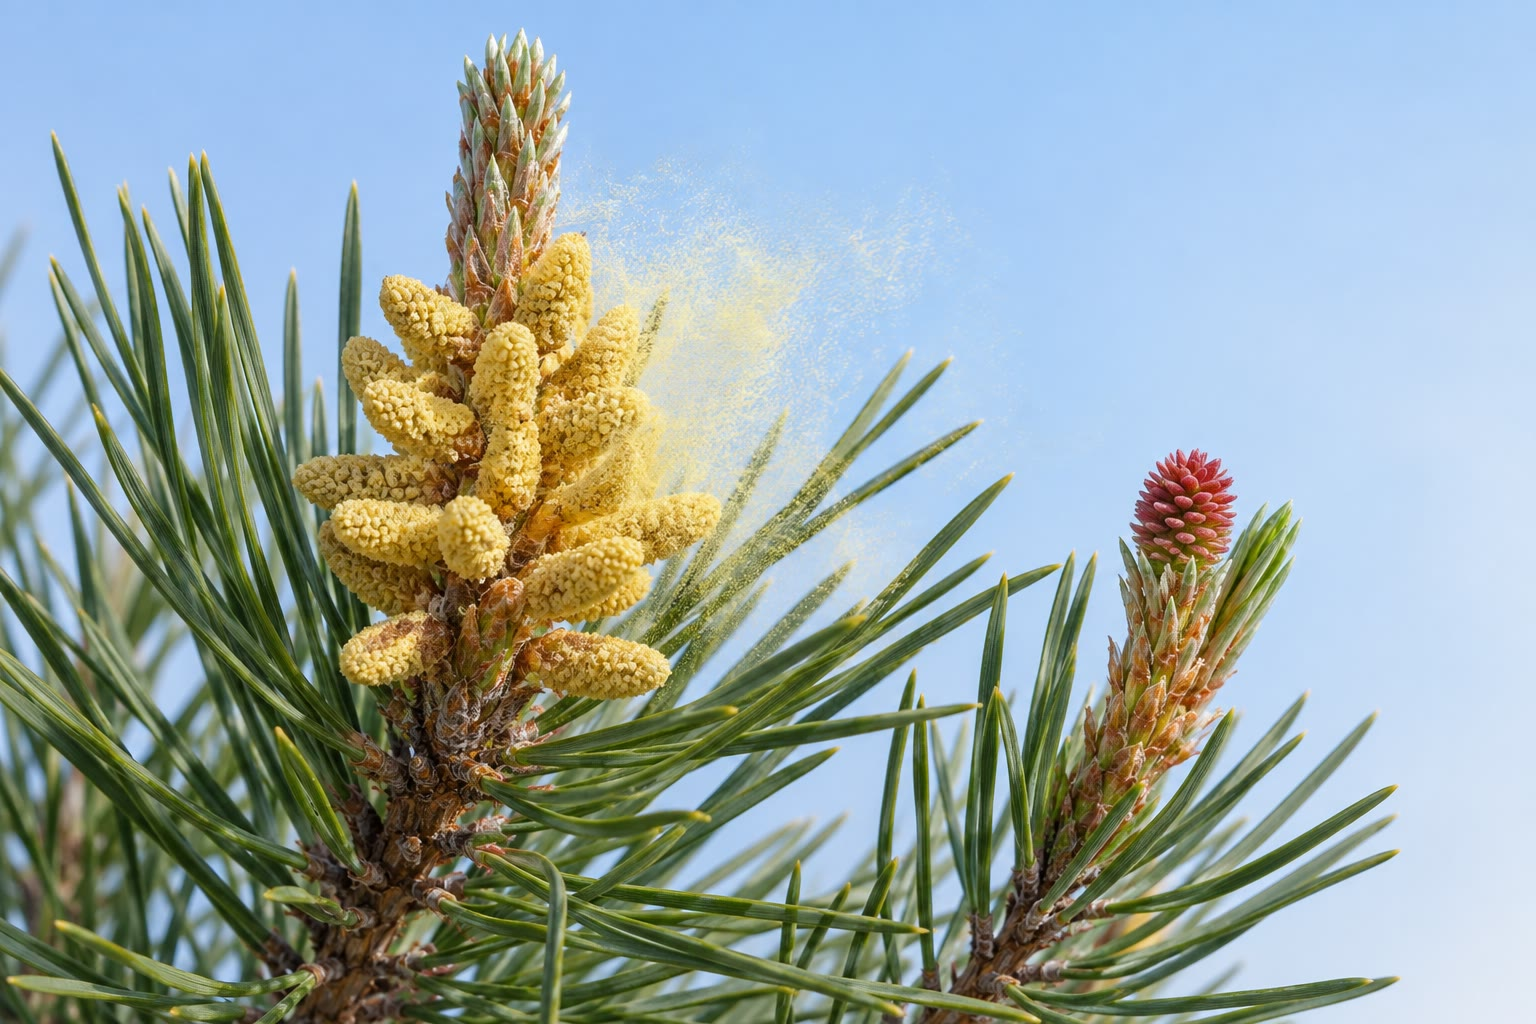
\includegraphics[width=0.6\linewidth]{images/book4/ai/b4-05-pine-cones.jpg}

{\small فرع صنوبر في الربيع: عنقود من المخاريط الذكرية الصفراء
تنثر \omterm{def:b2:plant-life-cycles:heterospory}{اللقاح}، ومخروط أنثوي أحمر صغير على طرف فرع آخر، حراشفه مفتوحة
لالتقاطه.}
\end{omfigure}

\begin{example}[اللقاح في الرياح]\label{ex:b2:plant-life-cycles:pollen}
حبة \omterm{def:b2:plant-life-cycles:heterospory}{لقاح} صنوبر، قطرها \qty{50}{\micro m} ولها مثانتان، تهبط بنحو
\qty{3}{cm/s}؛ وتطلق شجرة كبيرة نحو
$10^{11}$ حبة في الموسم، وهو ما يكفي لصبغ البرك صفراء. واحتمال أن
تحط حبة واحدة على \omterm{def:b2:plant-life-cycles:heterospory}{بييضة} بعينها ضئيل، ولا تنجح الاستراتيجية إلا
بالأعداد: فالإلقاح بالرياح رخيص في الحبة الواحدة، مكلف في عدد
الحبات، ومحصور في نباتات تنمو في غابات من نوعها ---
الصنوبريات، والنجيليات، والبلوط. أما النباتات الزهرية
(\cref{ch:b2:angiosperm-reproduction}) فوجدت طريقة لتسليم \omterm{def:b2:plant-life-cycles:heterospory}{اللقاح}
بالحيوانات، حبة واحدة في المرة إلى العنوان الصحيح.
\end{example}

\section{اتجاهات عبر النباتات اليابسة}

\begin{proposition}[أربعة اتجاهات]\label{prop:b2:plant-life-cycles:trends}
\index{انكماش الطور المشيجي}
من الطحالب إلى السراخس إلى النباتات البذرية: (1) ينمو \omterm{def:b2:plant-life-cycles:cycles}{الطور البوغي}
من ساق تابعة إلى النبات كله، وينكمش \omterm{def:b2:plant-life-cycles:cycles}{الطور المشيجي} من النبات إلى
حرشفة إلى بضع خلايا؛ (2) ويفسح تماثل الأبواغ المجال لتغايرها، ويبقى
\omterm{def:b2:plant-life-cycles:cycles}{الطور المشيجي} الأنثوي على الأم؛ (3) وينتقل الإلقاح من نطاف تسبح في
ماء السطح إلى أنبوب \omterm{def:b2:plant-life-cycles:heterospory}{لقاح}، فلا يعود التكاثر محتاجًا إلى مطر؛ (4)
وتنتقل وحدة الانتشار من البوغ --- خلية واحدة بمؤونة يوم --- إلى
البذرة، وهي جنين بغذاء وقشرة، تستطيع أن تنتظر. والجيل \omterm{def:b2:meiosis-heredity:meiosis}{الثنائي
الصيغة} مفضّل على اليابسة لأن الجسم \omterm{def:b2:meiosis-heredity:meiosis}{الثنائي الصيغة} يقنّع الطفرات
المتنحية، ويستطيع أن ينمو أكبر وأطول عمرًا بجملة وعائية، ولأن
البوغ المصنوع \omterm{def:b2:meiosis-heredity:meiosis}{بالتقسم المنصّف} على \omterm{def:b2:plant-life-cycles:cycles}{طور بوغي} عالٍ يسافر أبعد من عروس
تسبح من \omterm{def:b2:plant-life-cycles:cycles}{طور مشيجي} منخفض. ويستمر الاتجاه إلى النباتات الزهرية، حيث
يصير \omterm{def:b2:plant-life-cycles:cycles}{الطور المشيجي} الأنثوي سبع خلايا وتُلَفّ البذرة في ثمرة.
\end{proposition}

\begin{example}[مقارنة المجموعات]\label{ex:b2:plant-life-cycles:table}
\begin{center}
\small
\begin{tabular}{p{2.3cm}p{3.1cm}p{3.1cm}p{3.3cm}}
\hline
 & الطحالب & السراخس & الصنوبريات \\
\hline
الجيل \omterm{def:b2:meiosis-heredity:vocabulary}{السائد} & \omterm{def:b2:plant-life-cycles:cycles}{الطور المشيجي} & \omterm{def:b2:plant-life-cycles:cycles}{الطور البوغي} & \omterm{def:b2:plant-life-cycles:cycles}{الطور البوغي} \\
\omterm{def:b2:plant-life-cycles:cycles}{الطور المشيجي} & ساق مورقة، بقياس السنتيمتر & \omterm{def:b2:plant-life-cycles:fern}{مشيجة}، بقياس المليمتر، حرة & حبة \omterm{def:b2:plant-life-cycles:heterospory}{لقاح} (4 خلايا)؛ ومحتوى \omterm{def:b2:plant-life-cycles:heterospory}{البييضة} (آلاف الخلايا) \\
الأبواغ & صنف واحد & صنف واحد & أبواغ صغيرة وأبواغ كبيرة \\
الإلقاح & نطاف تسبح في الماء & نطاف تسبح في الماء & أنبوب \omterm{def:b2:plant-life-cycles:heterospory}{لقاح} \\
وحدة الانتشار & بوغ & بوغ & بذرة \\
النسيج الوعائي & لا شيء & خشب ولحاء & خشب ولحاء وخشب ثانوي \\
\hline
\end{tabular}
\end{center}
\end{example}

\section{تمارين}

\begin{exercise}[$\star$]\label{exo:b2:plant-life-cycles:1}
عرّف \omterm{def:b2:plant-life-cycles:cycles}{الطور المشيجي} \omterm{def:b2:plant-life-cycles:cycles}{والطور البوغي} والبوغ والعروس، وقل بأي نوع من
الانقسام (تقسم خيطي أم منصّف) يُنتج كل من الأربعة.
\end{exercise}

\begin{exercise}[$\star$]\label{exo:b2:plant-life-cycles:2}
\omterm{def:b2:plant-life-cycles:fern}{للسرخس} \emph{Ophioglossum reticulatum} عدد \num{1260}
صبغي في خلايا ورقته. فكم في بوغ، وفي خلية \omterm{def:b2:plant-life-cycles:fern}{مشيجة}، وفي نطفة، وفي
بويضة، وفي لاقحة؟
\end{exercise}

\begin{exercise}[$\star$]\label{exo:b2:plant-life-cycles:3}
أي جيل هي الوسادة الخضراء \omterm{def:b2:plant-life-cycles:moss}{لطحلب}؟ والساق البنية ذات المحفظة؟ وسعفة
\omterm{def:b2:plant-life-cycles:fern}{سرخس}؟ \omterm{def:b2:plant-life-cycles:fern}{والمشيجة}؟ وحبة \omterm{def:b2:plant-life-cycles:heterospory}{اللقاح}؟ ومخزون غذاء بذرة صنوبر؟ وجنين بذرة
صنوبر؟
\end{exercise}

\begin{exercise}[$\star$]\label{exo:b2:plant-life-cycles:4}
سمِّ أنماط \omterm{def:b2:plant-life-cycles:cycles}{دورة الحياة} الثلاثة وأعط كائنًا لكل منها. وأين يقع
\omterm{def:b2:meiosis-heredity:meiosis}{التقسم المنصّف} في كل منها؟
\end{exercise}

\begin{exercise}[$\star\star$]\label{exo:b2:plant-life-cycles:5}
تسبح نطفة \omterm{def:b2:plant-life-cycles:moss}{طحلب} بسرعة \qty{100}{\micro m/s}. فكم تستغرق لتبلغ رحمًا
يبعد \qty{3}{cm}؟ وغشاء ندى يتبخر خلال \qty{20}{min} بعد الشروق: فما
أقصى مدى للإلقاح؟ وعلّق على أقيسة مستعمرات الطحالب.
\end{exercise}

\begin{exercise}[$\star\star$]\label{exo:b2:plant-life-cycles:6}
احسب سرعة الترسيب في الهواء لبوغ \omterm{def:b2:plant-life-cycles:fern}{سرخس} نصف قطره
\qty{15}{\micro m} وكثافته \qty{1100}{kg/m^3} ($\eta =
\qty{1.8e-5}{Pa.s}$، $\rho_{\text{الهواء}} = \qty{1.2}{kg/m^3}$)،
والمسافة التي يقطعها من \qty{0.5}{m} في رياح سرعتها \qty{2}{m/s}.
وأعد ذلك من أجل بذرة صنوبر كتلتها \qty{5}{mg} يعطيها جناحها سرعة
هبوط \qty{0.8}{m/s}، تُطلق من \qty{20}{m}.
\end{exercise}

\begin{exercise}[$\star\star$]\label{exo:b2:plant-life-cycles:7}
تحمل سعفة \omterm{def:b2:plant-life-cycles:fern}{سرخس} \num{200} \omterm{def:b2:plant-life-cycles:fern}{بثرة} من \num{40} \omterm{def:b2:plant-life-cycles:fern}{حافظة بوغية}، وتصنع كل
حافظة \num{64} بوغًا. فكم بوغًا في السعفة؟ وإذا صار بوغ من كل
$10^{5}$ مشيجةً وأنتجت \omterm{def:b2:plant-life-cycles:fern}{مشيجة} من كل \num{50} طورًا بوغيًا، فكم سرخسًا
فتيًا تعطي السعفة؟
\end{exercise}

\begin{exercise}[$\star\star$]\label{exo:b2:plant-life-cycles:8}
اشرح لماذا يكون \omterm{def:b2:plant-life-cycles:heterospory}{تغاير الأبواغ} شرطًا مسبقًا للبذرة، ولماذا لا يستطيع
نبات متماثل الأبواغ أن يحيط طوره المشيجي الأنثوي \omterm{def:b2:plant-life-cycles:heterospory}{ببييضة}.
\end{exercise}

\begin{exercise}[$\star\star$]\label{exo:b2:plant-life-cycles:9}
قارن بوغ \omterm{def:b2:plant-life-cycles:fern}{سرخس} (كرة نصف قطرها \qty{15}{\micro m}، وكثافتها
\qty{1100}{kg/m^3}) ببذرة صنوبر (\qty{5}{mg}) بوصفهما وحدتي انتشار:
من جهة الكتلة، والمحتوى الطاقي (خذ \qty{20}{kJ/g} من المادة الجافة،
و\qty{50}{\%} جفافًا)، وما يستطيعه وما لا يستطيعه كل منهما عند الحط.
\end{exercise}

\begin{exercise}[$\star\star\star$]\label{exo:b2:plant-life-cycles:10}
ينثر صنوبر $10^{11}$ حبة \omterm{def:b2:plant-life-cycles:heterospory}{لقاح} فوق غابة؛ وعند ارتفاع البييضات تنتشر
الحبات في طبقة عمقها \qty{20}{m} فوق \qty{1}{km^2}. قدّر تركيز
\omterm{def:b2:plant-life-cycles:heterospory}{اللقاح} (حبات في المتر المكعب)، وعدد الحبات التي تمر في الثانية عبر
فتحة نقير \omterm{def:b2:plant-life-cycles:heterospory}{بييضة} (\qty{0.1}{mm^2}) في رياح سرعتها \qty{2}{m/s}،
والزمن اللازم لأن تتلقى \omterm{def:b2:plant-life-cycles:heterospory}{بييضة} حبة واحدة. فماذا يقول هذا عن توقيت
انفتاح المخاريط؟
\end{exercise}

\begin{exercise}[$\star\star\star$]\label{exo:b2:plant-life-cycles:11}
أعط ثلاثة أسباب لسيادة الجيل \omterm{def:b2:meiosis-heredity:meiosis}{الثنائي الصيغة} على \omterm{def:b2:plant-life-cycles:cycles}{دورة حياة} النباتات
اليابسة، وسببًا واحدًا لعدم اختفاء الجيل \omterm{def:b2:meiosis-heredity:meiosis}{الفردي الصيغة} بالكلية.
\end{exercise}

\begin{exercise}[$\star\star\star$]\label{exo:b2:plant-life-cycles:12}
عمل هوفمايستر قبل أن تُعرف الصبغيات. اشرح ما استطاع وما لم يستطع
إثباته عن \omterm{def:b2:plant-life-cycles:cycles}{تناوب الأجيال} بالمجهر والزرع وحدهما، وما الذي أضافه عدّ
الصبغيات.
\end{exercise}

\section{مسألة: من البوغ إلى البذرة}

\begin{problem}[{مسألة نهاية الأسبوع --- مقارنة حساب التكاثر عند
سرخس وصنوبر، من عدد الأبواغ وحبوب اللقاح إلى انتشارها، ومصير
الأطوار المشيجية، وكلفة البذرة، وتنتهي إلى عدد النواتج التكاثرية
التي على كل نبات صنعها لخلف واحد}]
\label{pb:b2:plant-life-cycles:1}
يحمل نبات \omterm{def:b2:plant-life-cycles:fern}{سرخس} \num{10} سعفات خصبة، في كل منها \num{200}
\omterm{def:b2:plant-life-cycles:fern}{بثرة} من \num{40} \omterm{def:b2:plant-life-cycles:fern}{حافظة بوغية} تصنع كل منها \num{64} بوغًا. والأبواغ:
نصف القطر \qty{15}{\micro m}، والكثافة \qty{1100}{kg/m^3}. ويُنتج
صنوبر ما في $2\times 10^{4}$ مخروط أنثوي من بييضات على مدى
حياته --- خذ \num{100} \omterm{def:b2:plant-life-cycles:heterospory}{بييضة} في المخروط --- و$10^{11}$ حبة \omterm{def:b2:plant-life-cycles:heterospory}{لقاح}
في السنة. والبذور: \qty{5}{mg}، منها \qty{50}{\%} مادة جافة عند
\qty{20}{kJ/g}. والهواء: $\eta = \qty{1.8e-5}{Pa.s}$، $\rho =
\qty{1.2}{kg/m^3}$؛ و$g = \qty{9.81}{m/s^2}$.

\medskip
\noindent\textbf{الجزء الأول --- أبواغ \omterm{def:b2:plant-life-cycles:fern}{السرخس}.}
\begin{enumerate}
  \item احسب عدد الأبواغ التي ينثرها النبات في الموسم.
  \item احسب كتلة بوغ واحد وكتلة المحصول كله.
  \item احسب سرعة ترسيب البوغ في الهواء.
  \item من سعف على \qty{0.5}{m} في رياح سرعتها \qty{1.5}{m/s}، كم
        تنتقل الأبواغ؟ وعلى أي مساحة (قرص بذلك النصف قطر) تنتشر،
        وكم يحط منها في المتر المربع؟
  \item اشرح لماذا يحمل الاضطراب قليلًا من الأبواغ أبعد بكثير، وما
        يعنيه هذا لاستعمار جزيرة جديدة.
  \item احسب المحتوى الطاقي لبوغ واحد (\qty{50}{\%} مادة جافة عند
        \qty{20}{kJ/g}) وللمحصول كله، وقارنه بطاقة بذرة صنوبر واحدة.
\end{enumerate}

\medskip
\noindent\textbf{الجزء الثاني --- الأطوار المشيجية.}
يحط بوغ من كل $2\times 10^{4}$ على تربة ندية بما يكفي لينمو
\omterm{def:b2:plant-life-cycles:fern}{مشيجة}؛ وتعيش \omterm{def:b2:plant-life-cycles:fern}{المشيجة} \num{6} أسابيع وتحتاج إلى ليلة رطبة ---
باحتمال $0.2$ في الأسبوع --- للإلقاح؛ وتعطي \omterm{def:b2:plant-life-cycles:fern}{المشيجة} الملقحة طورًا
بوغيًا فتيًا باحتمال
$0.5$؛ وينجو \omterm{def:b2:plant-life-cycles:cycles}{الطور البوغي} الفتي إلى البلوغ باحتمال
$0.02$.
\begin{enumerate}[resume]
  \item كم \omterm{def:b2:plant-life-cycles:fern}{مشيجة} ينتج محصول النبات؟
  \item احسب احتمال أن تمر \omterm{def:b2:plant-life-cycles:fern}{المشيجة} بليلة رطبة واحدة على الأقل في
        أسابيعها الستة.
  \item احسب العدد المنتظر من السراخس البالغة التي ينتجها محصول
        موسم واحد.
  \item إذا عاش النبات الأم \num{30} سنة، فكم خلفًا بالغًا يترك،
        وماذا يقول هذا عن جمهرة \omterm{def:b2:plant-life-cycles:fern}{السرخس}؟
  \item تسبح نطفة \omterm{def:b2:plant-life-cycles:fern}{سرخس} بسرعة \qty{100}{\micro m/s}، وأرحام \omterm{def:b2:plant-life-cycles:fern}{المشيجة}
        تبعد \qty{1}{mm} عن مذاريها. فكم يستغرق الإلقاح الذاتي؟
        ولماذا تتجنبه سراخس كثيرة مع ذلك (أعط آلية واحدة)؟
  \item بأي معنى تكون \omterm{def:b2:plant-life-cycles:fern}{المشيجة} الحلقة الضعيفة في دورة \omterm{def:b2:plant-life-cycles:fern}{السرخس}؟
\end{enumerate}

\medskip
\noindent\textbf{الجزء الثالث --- \omterm{def:b2:plant-life-cycles:heterospory}{لقاح} الصنوبر.}
\begin{enumerate}[resume]
  \item حبة \omterm{def:b2:plant-life-cycles:heterospory}{اللقاح} كرة نصف قطرها \qty{25}{\micro m} كثافتها الفعلية
        \qty{600}{kg/m^3} (بحساب مثانتي الهواء).
        احسب سرعة ترسيبها.
  \item من مخروط على \qty{15}{m} في رياح سرعتها \qty{3}{m/s}، كم
        تنتقل؟
  \item تنتشر الحبات $10^{11}$ في \qty{1}{km^2} من الغابة إلى عمق
        \qty{20}{m}. احسب التركيز.
  \item يقدّم النقير فتحة \qty{0.1}{mm^2} إلى رياح
        سرعتها \qty{2}{m/s}. احسب عدد الحبات الداخلة إليه في
        الساعة، والزمن اللازم لتلقّي أول حبة.
  \item اشرح لماذا لا يعقد صنوبر منفرد يبعد \qty{5}{km} عن الغابة
        بذورًا تُذكر، ولماذا تنمو الأنواع الملقحة بالرياح في غابات.
  \item قارن الأعداد: كم حبة \omterm{def:b2:plant-life-cycles:heterospory}{لقاح} تصنع الغابة لكل \omterm{def:b2:plant-life-cycles:heterospory}{بييضة}، إذا ضمت
        \num{1000} صنوبرة في كل منها \num{2000} \omterm{def:b2:plant-life-cycles:heterospory}{بييضة}؟
\end{enumerate}

\medskip
\noindent\textbf{الجزء الرابع --- بذور الصنوبر.}
من بييضات الشجرة، تُلقَّح \qty{60}{\%} وتملأ \qty{80}{\%} من هذه
بذرة؛ وتصير البذرة بادرة باحتمال $0.05$
وتصير البادرة بالغة باحتمال $0.01$.
\begin{enumerate}[resume]
  \item احسب عدد البذور التي تصنعها الشجرة في حياتها، وكتلتها
        وطاقتها الكليتين.
  \item تهبط البذرة المجنحة بسرعة \qty{0.8}{m/s}. فمن \qty{20}{m} في
        رياح سرعتها \qty{3}{m/s}، كم تنتقل؟ وقارن ذلك
        \omterm{def:b2:plant-life-cycles:heterospory}{باللقاح}.
  \item احسب العدد المنتظر من الخلف البالغ، وقارنه بخلف \omterm{def:b2:plant-life-cycles:fern}{السرخس}.
  \item احسب الطاقة التي تستثمرها الشجرة في كل خلف بالغ، والتي
        يستثمرها \omterm{def:b2:plant-life-cycles:fern}{السرخس} في كل خلف بالغ (بالأبواغ وحدها)، وقارن.
  \item يستطيع بوغ \omterm{def:b2:plant-life-cycles:fern}{السرخس} أن ينتظر بضعة أسابيع، وبذرة الصنوبر عدة
        سنوات. اشرح، بأرقام الطاقة، لماذا تحتمل البذرة السكون ولا
        يحتمله البوغ.
  \item أعط ميزتين تجعلان البذرة جديرة بكلفتها وشرطين تكون
        استراتيجية \omterm{def:b2:plant-life-cycles:fern}{السرخس} فيهما أفضل.
  \item اذكر النتيجة: عدد النواتج التكاثرية لكل خلف بالغ عند
        \omterm{def:b2:plant-life-cycles:fern}{السرخس} وعند الصنوبر، والطاقة التي ينفقها كل منهما لكل خلف
        بالغ.
\end{enumerate}
\end{problem}
